\section{\textsc{Omelette tomo}}

\subsection*{Ingredients for 1 omelette:}

\begin{tabular}{p{7.5cm} p{7.5cm}}
	& \\
	4 eggs & 5 Cherrytomatoes \\
	2ts butter & 200g mozzarella \\
	salt & pepper \\
	basil to taste &
\end{tabular}

\subsection*{Serving suggestion:}

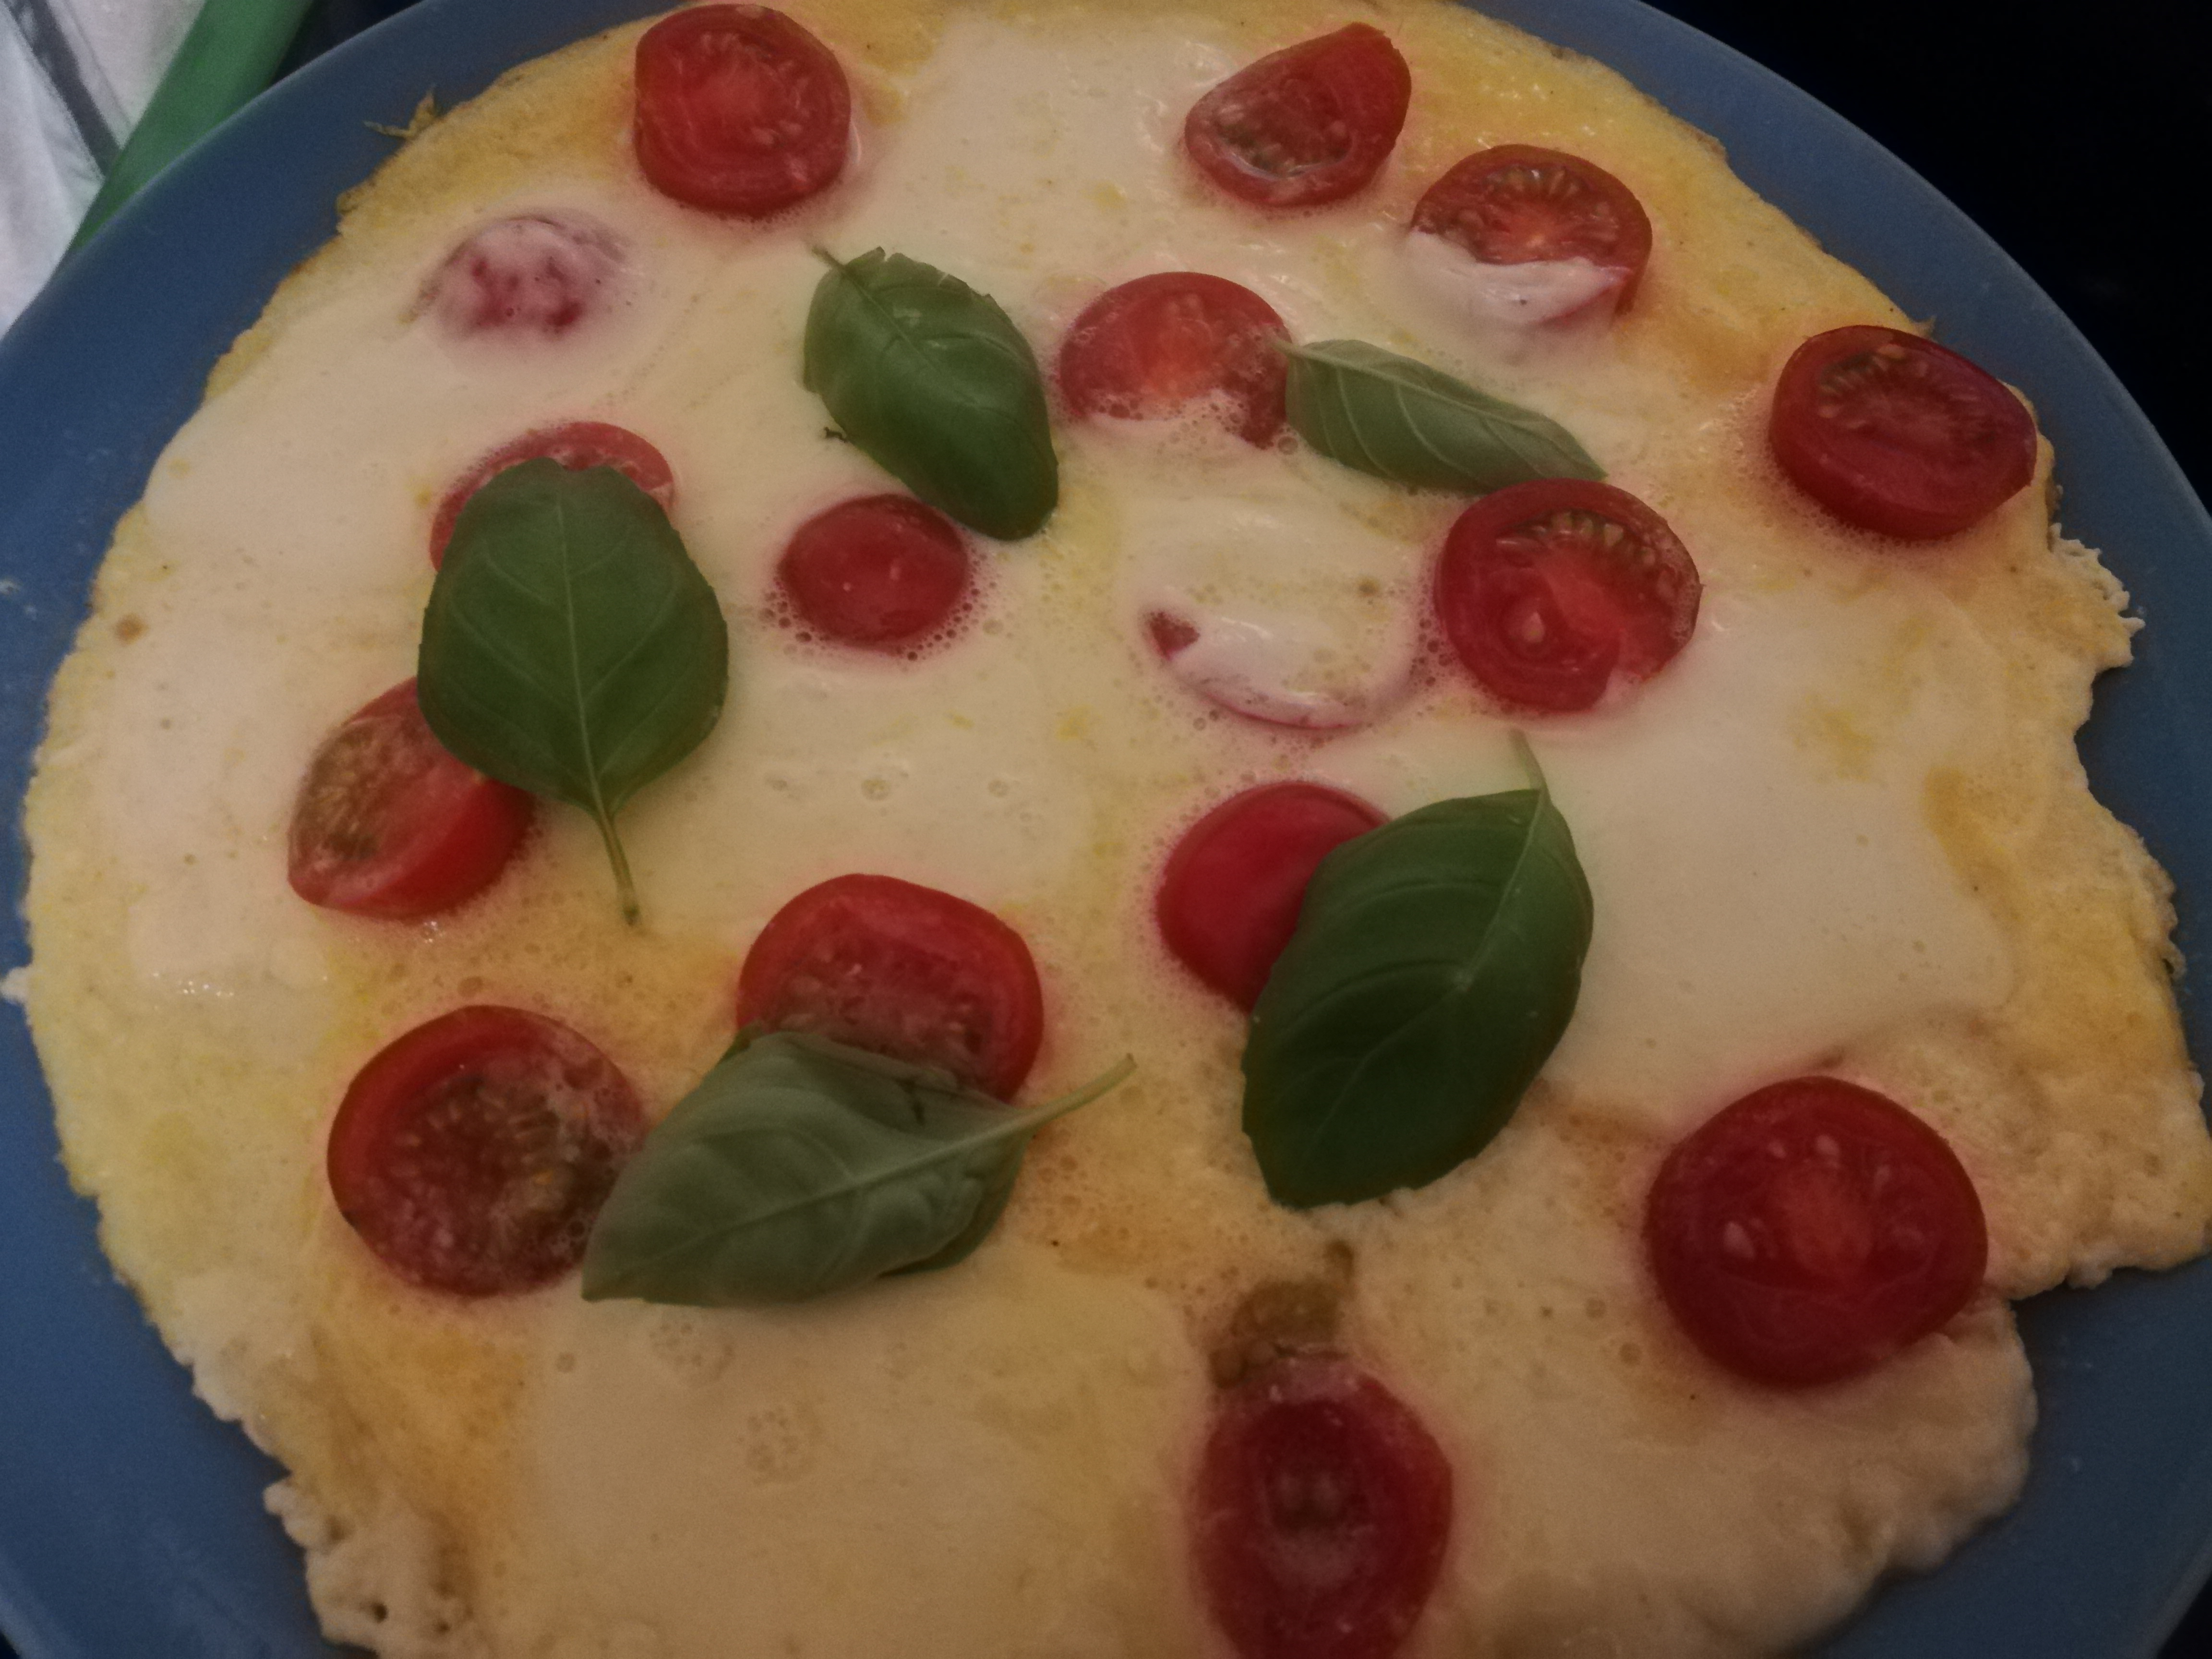
\includegraphics[width=\textwidth]{img/omlett/omlett_tomo_fertig.jpg} \cite{omlettomo}

\subsection*{How it's done:}

\begin{tabular}{p{15cm}}
	\\
  Beat the eggs with a whisk until it is foamy.\\
  Add salt and pepper to taste.\\
  Melt the butter in a pan.\\
  Pour the egg mixture into the pan and let it set over a high heat.\\
  Spread the mozzarella and the tomatoes on it.\\
  Fry with a lid on a low heat for 5 minutes.\\
  Place it on a large plate and decorate it with basil.
\end{tabular}
